%*******************************************************************************
%*********************************** First Chapter *****************************
%*******************************************************************************

\chapter{Introduction}  %Title of the First Chapter

\ifpdf
    \graphicspath{{Chapter1/Figs/Raster/}{Chapter1/Figs/PDF/}{Chapter1/Figs/}}
\else
    \graphicspath{{Chapter1/Figs/Vector/}{Chapter1/Figs/}}
\fi

Gallium nitride \nomenclature[z-GaN]{GaN}{Gallium Nitride} (GaN) has been termed the 'most important semiconductor material since silicon' \cite{Humphreys2008}, and indeed the influence of this incredible material and it's associated alloys (termed III-nitrides) is pervasive in modern society. The impact of III-nitride materials is perhaps best evidenced by the global transition from traditional lighting sources to semiconductor lighting solutions based on III-nitride materials. Since the first demonstration of a high-brightness blue light emitting diode \nomenclature[z-LED]{LED}{Light-Emitting Diode} (LED) in 1991 by Shuji Nakamura \cite{Nakamura1991}, the widespread use of LEDs for general lighting purposes has blossomed into a multi-billion pound industry. The extraordinary optical properties of III-nitride materials have enabled their application outside of the lighting industry: the development of III-nitride based lasers has found applications in telecommunications \cite{Najda2015}, medicine \cite{BerlienBreuerMuellerEtAl2012} and data storage . Furthermore, III-nitride optical emitters have been used as single photon sources \nomenclature[z-SPS]{SPS}{Single Photon Source} (SPSs) which have applications in cryptography for secure communications \cite{Kako2006}.
\\The optoelectronic properties of III-nitride materials are somewhat astonishing: GaN suffers from a defect density several orders of magnitude higher than other optically active semiconductor materials such as gallium arsenide \nomenclature[z-GaAs]{GaAs}{Gallium Arsenide} (GaAs) \cite{Bennett2010b} yet is still optically active. Despite this, the effects of defects originating from the heteropitaxial growth of GaN are clearly deleterious when considering III-nitride device operation. 
This work aims to explore the manner in which the microstructural properties of photonic III-nitride devices affect their performance by combining multiple microscopy techniques, an approach we term 'multi-microscopy', thus allowing us to link specific structural features with emissive properties at the device level. The experimental research in this thesis is separated into four main sections. 
\\The first section details the investigation of inhomogeneous electroluminescence \nomenclature[z-EL]{EL}{Electroluminescence} (EL) of indium gallium nitride (InGaN) quantum well (QW) LEDs. By employing the use of scanning probe techniques, electron microscopy and spectroscopy the underpinning cause of LED behaviour was elucidated and reported.
\\The second section involves microscopy-based investigation into the mechanisms behind incomplete etching in the fabrication of III-nitride based microdisk cavities and the effect of this issue on the overall optical performance of these cavities
\\The third section describes the microscopy of one dimensional \nomenclature[z-1-D]{1-D}{One-Dimensional} (1-D) photonic crystal cavity (PCC) 'nanobeam' cavities. The intrinsic resistance of III-nitride based materials can often result in improperly etched features, which can results in high optical losses in cavities. This section concerns the use of tomographic techniques such as electron tomography \nomenclature[z-ET]{ET}{Electron Tomography} (ET) and focussed ion beam tomography \nomenclature[z-FIBT]{FIBT}{Focussed Ion Beam Tomography} (FIB-T) to investigate the effect of these issues on the emission of III-nitride nanobeam cavities. 

%********************************** %First Section  **************************************
\section{III-Nitride Material Properties } %Section - 1.1 

\subsection{Crystal Structure}
\label{section1.1.1}

GaN can crystallise into two distinct crystal structures: hexagonal (wurtzite) and cubic (zinc blende and rock salt). Under ambient conditions, wurtzite GaN is the most commonly studied form as it is the most structurally stable. Thus, the work discussed in this thesis concerns wurtzite III-nitrides. A schematic of a wurtzite III-nitride crystal structure is shown in Fig.\ref{1.1} and consists of stacked hexagonal close-packed planes following an ABABAB stacking sequence. Atoms of the respective elements are tetrahedrally bonded to one another. However, in the case of III-nitrides this structure deviates from ideal tetrahedral bonding and results in a non-zero dipole moment for each unit cell which will be discussed in the following sections.
\\ A 4-index Miller-Bravais notation (hkil) is used to denote the crystal planes where the index {\it i} is defined by the relation:

\begin{equation}
 i = -(h+k)
 \end{equation}
\\
 
The crystallographic planes (0001), (1-100) and (11-20) shown in Fig.\ref{1.1} are often termed the {\it c}, {\it m} and {\it a}-planes in the literature. The fundamental unit cell of the wurtzite GaN crystal structure and its associated lattice parameters \textbf{a} and \textbf{c} is shown in Fig.\ref{1.2}

\begin{figure}[h]
	\centering
	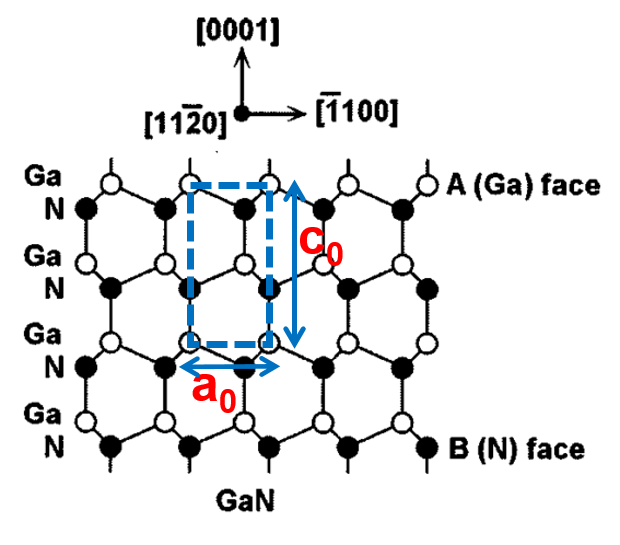
\includegraphics[width=0.5\textwidth]{Figs/Ch1/unit_cell.png}
	\caption {Unit cell (dashed line) for GaN crystal structure and lattice parameters $\mathbf{a_{0}},\mathbf{c_{0}}$. Adapted from \cite{Yu1999}}
	\label{1.2}
\end{figure}
\FloatBarrier

Other members of the III-nitride materials such as indium nitride \nomenclature[z-InN]{InN}{Indium Nitride} (InN) or aluminium nitride \nomenclature[z-AlN]{AlN}{Aluminium Nitride} (AlN) have different lattice parameters due to the differing atomic radii of aluminium and indium relative to gallium.

\begin{table}[!htb]
	\centering
	\label{tab1.1}
	\begin{tabular}{ccc}
		Alloy & \textbf{a} (\si{\angstrom}) at T = 300K & \textbf{c} (\si{\angstrom}) at T = 300K \\
		%heading
		\hline\hline
		GaN   & 3.189   & 5.185   \\
		InN   & 3.545   & 5.703   \\
		AlN   & 3.112  & 4.982  \\ 
		\hline
	\end{tabular}
	\caption{Room temperature lattice parameters for GaN, InN and AlN \cite{Vurgaftman2003}.}
\end{table}

III-nitride photonic devices are often heterostructures consisting of ternary alloys the materials shown in Table~\ref{tab1.1}. Lattice parameters of a relaxed ternary alloy $A_{x}B_{1-x}N$ can be estimated using Vegard's law \cite{Vickers2003}:

\begin{equation}
\mathbf{a} = x \mathbf{a}_{AN} + (1-x)\mathbf{a}_{BN}
\end{equation}

\begin{equation}
\mathbf{c} = x \mathbf{c}_{AN} + (1-x)\mathbf{c}_{BN}
\end{equation}

Typical indium compositions for blue LEDs range between 15-20 $\%$, which leads to a considerable lattice mismatch of approximately 2 $\%$, resulting in considerable amounts of strain in these GaN/InGaN heterostructures.

\subsection{Band Structure} 
\label{section1.1.2}

One of the principal driving factors behind the interest in III-nitrides for photonic devices is their direct bandgap which collectively spans the visible spectrum and beyond.


\subsection{Built-in Fields} 
\label{section1.1.3}
III-nitride materials in wurtzite structure are termed 'polar' materials, due to the fact they exhibit a spontaneous polarisation field \cite{Ambacher2002}. This occurs due to III-nitride bonding structure deviating from an ideal tetrahedral structure along the (0001) axis along the crystal, combined with the ionicity of the bond \cite{Ren2015}. This deviation causes each unit cell to possess a non-zero dipole moment along the principal axis of the tetrahedral bonding structure, resulting in an overall spontaneous polarization in the crystal. As the III-nitride wurtzite structure is non-centrosymmetric, the direction of the polarization depends on whether the crystal exhibits (+ {\it c}) or (-{\it c}) polarity, as shown in Fig.\ref{1.3}

\begin{figure}[h]
	\centering
	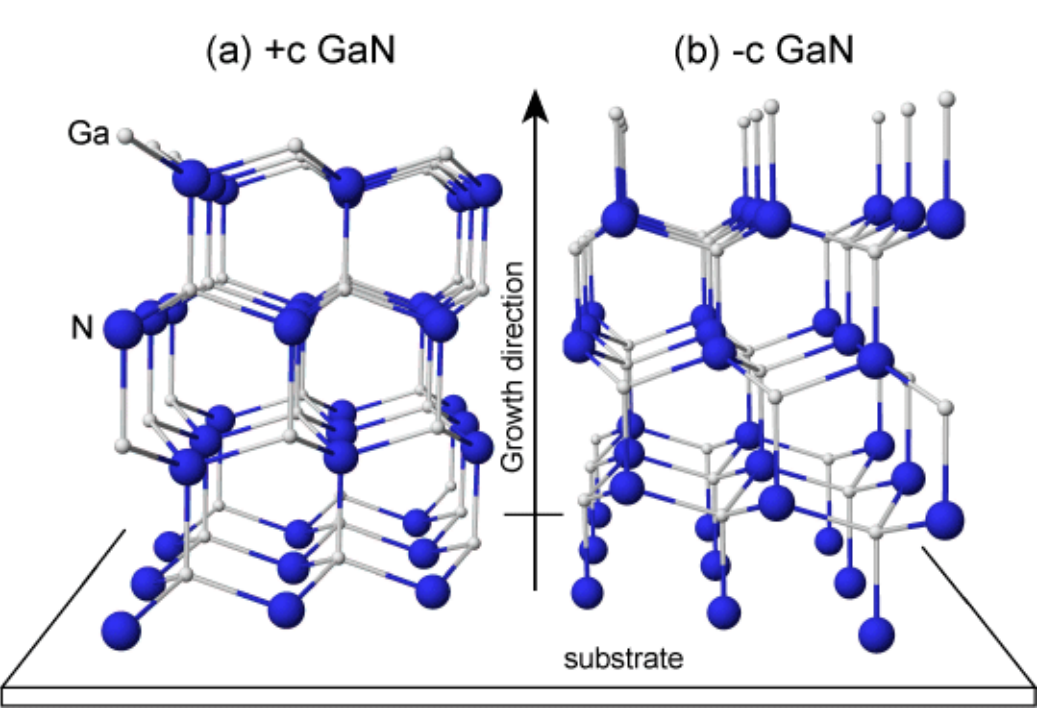
\includegraphics[width=0.5\textwidth]{Figs/Ch1/p2.png}
	\caption {Illustration of Ga-face (+ {\it c}) and N-face (-{\it c}) GaN wrutzite crystal exhibiting polarity along the {\it c}-axis \cite{Sumiya2004}.}
	\label{1.3}
\end{figure}
\FloatBarrier

This non-zero dipole moment is particularly strong for III-nitrides relative to other III-V semiconductors due to the strong electronegativity and small size of nitrogen compared to other group V elements, resulting in a metal-nitrogen bond with greater ionicity than other III-V bonds \cite{wood2007polarization}. Fig.\ref{1.4} shows a GaN unit cell with lattice parameters {\textbf {\it c}} and \textbf{\it a} denoted.

\begin{figure}[h]
	\centering
	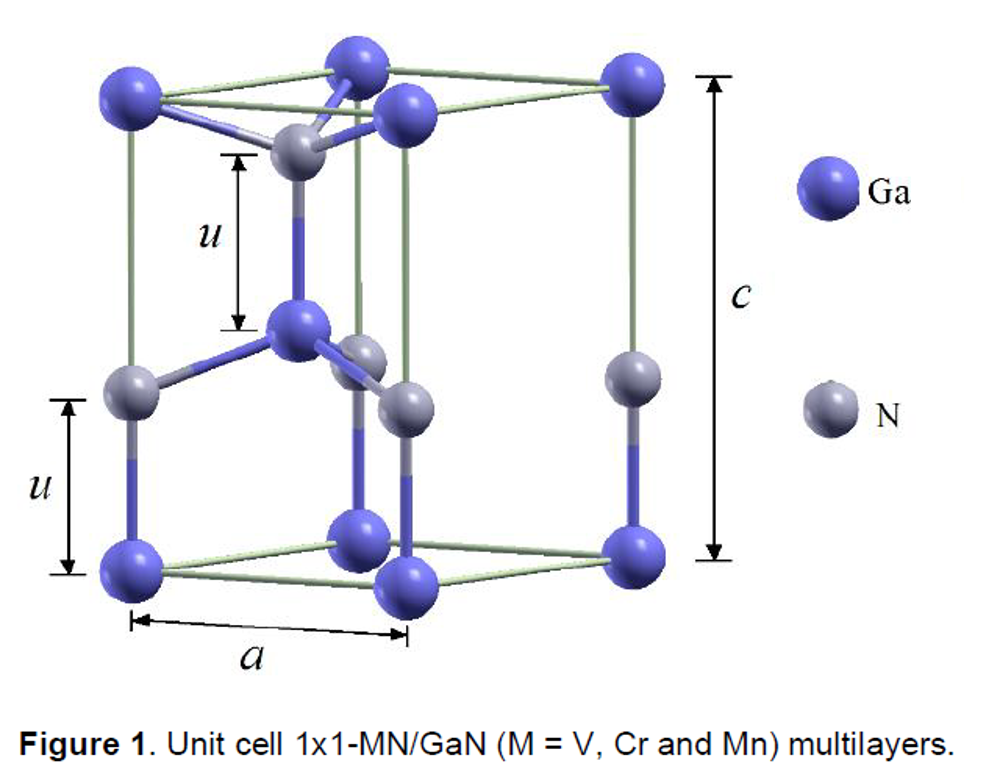
\includegraphics[width=0.5\textwidth]{Figs/Ch1/2unit.png}
	\caption {GaN unit cell with lattice parameters \textbf{\it c} and \textbf{\it a} \cite{Miguel2014}}
	\label{1.4}
\end{figure}
\FloatBarrier 

If all nearest neighbour bond lengths are equal, an ideal hexagonal closed packed crystal exhibiting zero spontaneous polarisation would have a ratio of lattice parameters denoted by:

\begin{equation}
\frac{c}{a}= (\frac{8}{3})^{0.5} = 1.63299
\end{equation} 

The degree of spontaneous polarisation observed in III-nitride materials is thus determined by the amount their lattice parameter ratio deviates from this ideal value. The values for bulk III-nitride materials are given in Table.\ref{tab1.2}. 

\begin{table}[!htb]
	\centering
	\label{tab1.1}
	\begin{tabular}{cc}
		\textbf{Alloy} &  $\mathbf{\frac{c}{a}}$ \\
		%heading
		\hline\hline\\
		GaN   & 1.6259      \\
		InN   & 1.6116     \\
		AlN   & 1.6010   \\ 
		\hline
	\end{tabular}
	\caption{Bulk $\frac{c}{a}$ ratios for GaN, InN and AlN \cite{Ren2015}.}
	\label{tab1.2}
\end{table}

A lower $\mathbf{\frac{c}{a}}$ ratio indicates a higher angle between the three bonds at the base of the tetrahedral bonding structure, resulting in a lower compensation polarisation along the (0001) axis and a higher spontaneous polarisation. Thus according to Table.\ref{tab1.2} the strongest spontaneous polarisation is observed in AlN and the weakest in GaN.\\
It is important to note that materials which exhibit spontaneous polarisation also exhibit piezoelectric polarisation \cite{Ambacher2002}. Strain experienced by the material results in the distortion in of the crystal lattice, which can either alleviate or exacerbate the deviation from the ideal tetrahedral structure resulting in an additional polarisation. This piezoelectric polarization is a crucial consideration in III-nitride devices which often consist of QW heterostructures: lattice mismatches with underlying layers result in the expansion or contraction of III-nitride films. Interestingly two different polarisation configurations are obtained for AlGaN and InGaN coherently strained to GaN. In the case of InGaN the piezoelectric field acts against the spontaneous field, whilst the opposite is true for AlGaN strained to GaN. Within the context of visible light LEDs, InGaN containing QWs are dominated by the piezoelectric contribution to the polarization fields \cite{Fiorentini1999} due to the sizeable lattice mismatch between GaN and InN ($~11\%$) \cite{Chichibu2006}.

\subsubsection{The Quantum Confined Stark Effect}

As previously discussed, III-nitride photonic devices often make use of heterostructures known as quantum wells, which enhance radiative efficiency by confining carrier wavefunctions over a range of several nanometres. Given the presence of built-in fields in III-nitride materials, it is important to consider the effect polarisation fields will have on the band structure and thus optical properties of quantum wells as shown in Fig.\ref{1.5}

\begin{figure}[h]
	\centering
	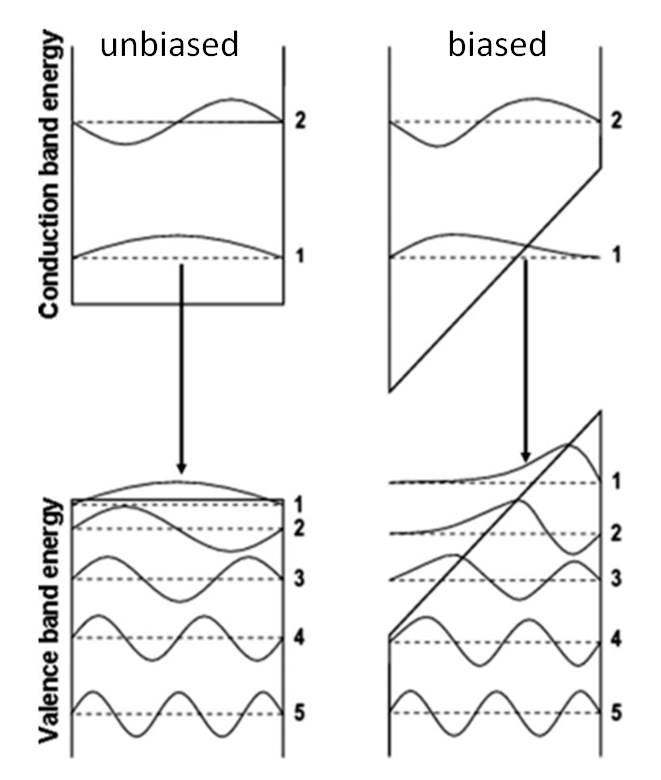
\includegraphics[width=0.5\textwidth]{Figs/Ch1/QCSE.png}
	\caption {Unbiased and biased quantum well energy levels with associated carrier wavefunctions. Under an applied field the overlap between the electron and hole carrier wavefunctions is reduced \cite{Ryou2009}.}
	\label{1.5}
\end{figure}
\FloatBarrier 

The transition from a rectangular to a 'sawtooth'-shaped potential well results in the reduction in energy of the optical transition, meaning the photons emitted from the QW are red-shifted. However, as the carrier density within the QW is increased, by either optical or electrical injection, the polarization fields are effectively screened resulting in a carrier density-dependent optical transition energy.\\
A further effect of the polarization fields is to spatially separate the carrier wave functions, thus reducing their overlap as shown in Fig.\ref{1.5}. This results in a reduced probability for the radiative recombination carriers thus reducing the efficiency of III-nitride QW emitters.
\subsection{Defects in III-nitrides}  %Section - 1.4 
\label{section1.1.4}

%********************************** %Second Section  **************************************
\section{III-nitride Cavities } %Section - 1.1 

\subsection{Cavity characteristics}

\subsection{Cavity Designs}

